\section{Kernel optimizations}

\begin{frame}[fragile]
\frametitle{Measure - Kernel initialization functions}
To find out which kernel initialization functions are the longest to
execute, add \code{initcall_debug} to the kernel command line.
Here's what you get on the kernel log:
\begin{block}{}
\tiny
\begin{verbatim}
...
[    3.750000] calling  ov2640_i2c_driver_init+0x0/0x10 @ 1
[    3.760000] initcall ov2640_i2c_driver_init+0x0/0x10 returned 0 after 544 usecs
[    3.760000] calling  at91sam9x5_video_init+0x0/0x14 @ 1
[    3.760000] at91sam9x5-video f0030340.lcdheo1: video device registered @ 0xe0d3e340, irq = 24
[    3.770000] initcall at91sam9x5_video_init+0x0/0x14 returned 0 after 10388 usecs
[    3.770000] calling  gspca_init+0x0/0x18 @ 1
[    3.770000] gspca_main: v2.14.0 registered
[    3.770000] initcall gspca_init+0x0/0x18 returned 0 after 3966 usecs
...
\end{verbatim}
\end{block}
You might need to increase the log buffer size with
\kconfig{CONFIG_LOG_BUF_SHIFT} in your kernel configuration. You will
also need \kconfig{CONFIG_PRINTK_TIME} and \kconfig{CONFIG_KALLSYMS}.
\end{frame}

\begin{frame}
\frametitle{Kernel boot graph}
With \code{initcall_debug}, you can generate a boot graph
making it easy to see which kernel initialization functions
take most time to execute.
\begin{itemize}
\item Copy and paste the output of
      the \code{dmesg} command to a file (let's call it \code{boot.log})
\item On your workstation, run the \code{scripts/bootgraph.pl} script
      in the kernel sources: \\
      \code{scripts/bootgraph.pl boot.log > boot.svg}
\item You can now open the boot graph with a vector graphics
      editor such as \code{inkscape}:
\end{itemize}
\begin{center}
    \includegraphics[width=\textwidth]{slides/boot-time-kernel/boot.pdf}
\end{center}
\end{frame}

\begin{frame}
\frametitle{Using the kernel boot graph (1)}
Start working on the functions consuming most time first. For each
function:
\begin{itemize}
\item Look for its definition in the kernel source code. You can use
      Elixir (for example \url{https://elixir.bootlin.com}).
\item Be careful: some function names don't exist, the names
      correspond to {\em modulename}\code{_init}. Then, look for
      initialization code in the corresponding module.
\item Remove unnecessary functionality:
      \begin{itemize}
      \item Find which kernel configuration parameter
      compiles the code, by looking at the Makefile in the corresponding
      source directory.
      \end{itemize}
\end{itemize}
\end{frame}

\begin{frame}
\frametitle{Using the kernel boot graph (2)}
\begin{itemize}
\item Postpone:
      \begin{itemize}
      \item Find which module (if any) the function belongs to.
            Load this module later if possible.
      \end{itemize}
\item Optimize necessary functionality:
      \begin{itemize}
      \item Look for parameters which could be used to reduce probe time,
            looking for the \code{module_param} macro.
      \item Look for delay loops and calls to functions containing
            \code{delay} in their name, which could take more time than
            needed. You could reduce such delays, and see whether the
            code still works or not.
      \end{itemize}
\end{itemize}
\end{frame}

\begin{frame}
\frametitle{Reduce kernel size}
First, we focus on reducing the size without removing features
\begin{itemize}
	\item The main mechanism is to use kernel modules
	\item Compile everything that is not needed at boot time as a
		module
	\item Two benefits: the kernel will be smaller and load faster, and
		less initialization code will get executed
	\item Remove features that are not used by userland:
		\kconfig{CONFIG_KALLSYMS}, \kconfig{CONFIG_DEBUG_FS},
		\kconfig{CONFIG_BUG}
	\item Use features designed for embedded systems:
		\kconfig{CONFIG_SLOB}, \kconfig{CONFIG_EMBEDDED}
\end{itemize}
\end{frame}

\begin{frame}
\frametitle{Kernel Compression}
Depending on the balance between your storage reading speed and your
CPU power to decompress the kernel, you will need to benchmark
different compression algorithms.

Also recommended to experiment with compression options at the
end of the kernel optimization process, as the results may vary
according to the kernel size.
\begin{center}
    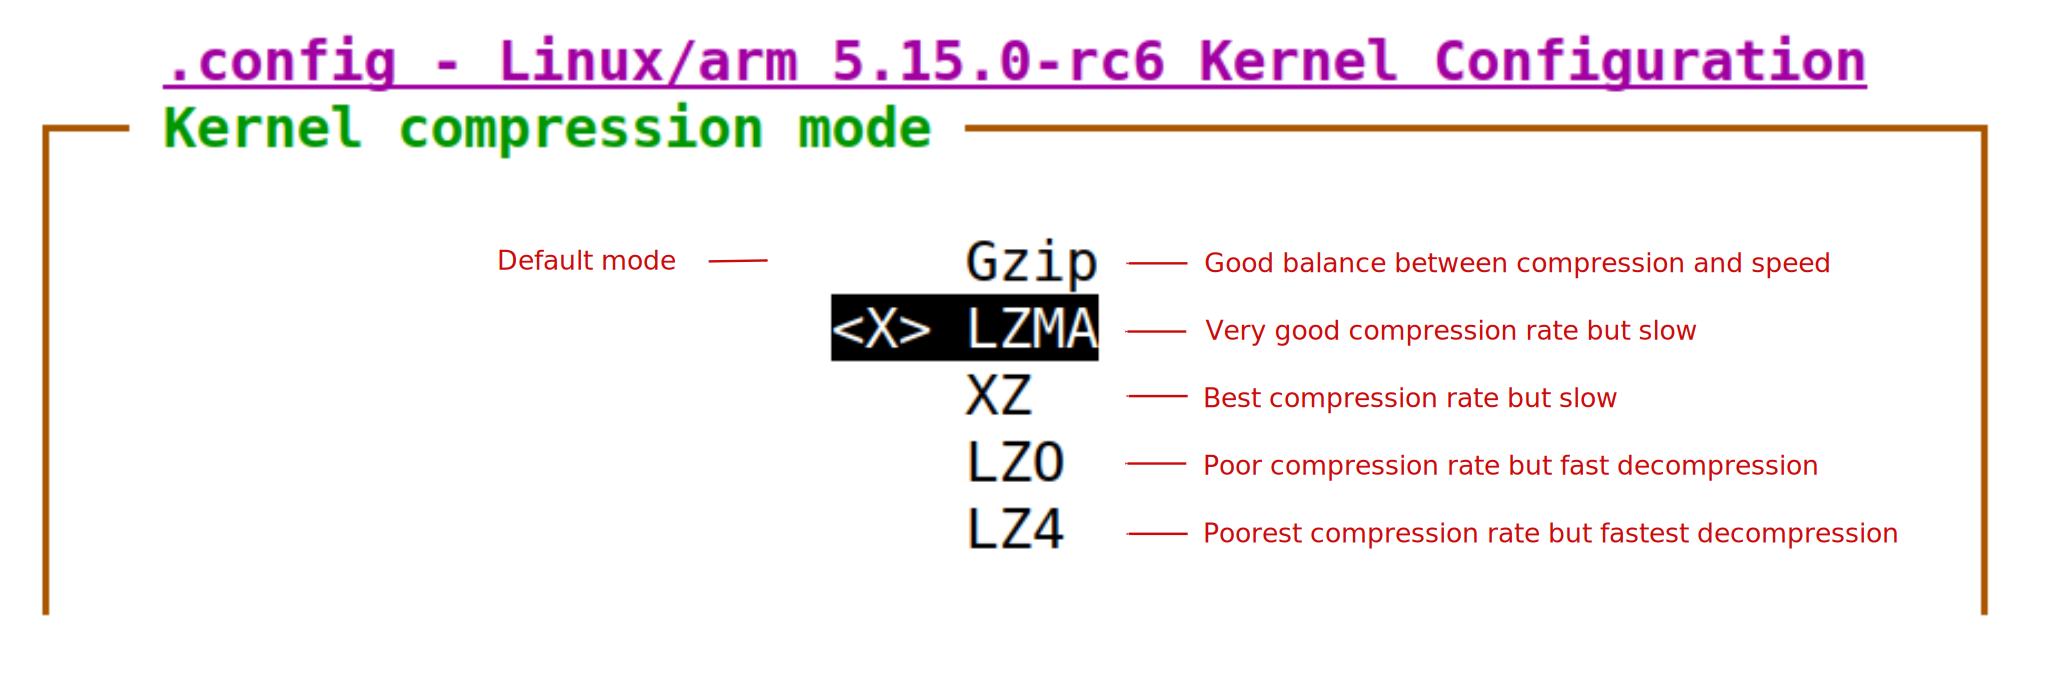
\includegraphics[width=\textwidth]{slides/boot-time-kernel/kernel-compression-options.pdf}
\end{center}
\end{frame}

\begin{frame}
\frametitle{Kernel compression options}
Results on TI AM335x (ARM), 1 GHz, Linux 5.1
{\fontsize{7}{10}\selectfont
\begin{tabular}{| l || c | c | c | c | c |}
\hline
Timestamp & gzip & lzma & xz & lzo & lz4 \\
\hline
Size & 2350336 & 1777000 & {\bf 1720120} & 2533872 & 2716752 \\
Copy & 0.208 s & 0.158 s & {\bf 0.154 s} & 0.224 s & 0.241 s \\
Time to userspace & 1.451 s & 2.167 s & 1.999s & {\bf 1.416 s} & 1.462 s \\
\hline
\end{tabular}
}
\vfill{}
Gzip is close. It's time to try with faster storage (SanDisk Extreme
Class A1)
{\fontsize{7}{10}\selectfont
\begin{tabular}{| l || c | c | c | c | c |}
\hline
Timestamp & gzip & lzma & xz & lzo & lz4 \\
\hline
Size & 2350336 & 1777000 & {\bf 1720120} & 2533872 & 2716752 \\
Copy & 0.150 s & 0.114 s & {\bf 0.111 s} & 0.161 s & 0.173 s \\
Time to userspace & 1.403 s & 2.132 s & 1.965 s & {\bf 1.363 s} & 1.404 s \\
\hline
\end{tabular}
}
\newline\newline
Lzo and Gzip seem the best solutions. Always benchmark as the results
depend on storage and CPU performance.
\end{frame}

\begin{frame}[fragile]
\frametitle{Compressing the kernel with Zstandard}
\begin{itemize}
  \item Zstandard is a relatively recent compression scheme, implemented
        by Yann Collet.
  \item Unfortunately, not available on ARM yet.\\
        Only on x86, mips and s390 (Linux 5.15 status).
  \item Compressing better than gzip and decompressing as fast as LZO,
        it could be the best option.
  \item See \url{https://en.wikipedia.org/wiki/Zstandard}
\end{itemize}
\begin{block}{}
\small
\begin{verbatim}
config KERNEL_ZSTD
        bool "ZSTD"
        depends on HAVE_KERNEL_ZSTD
        help
          ZSTD is a compression algorithm targeting intermediate compression
          with fast decompression speed. It will compress better than GZIP and
          decompress around the same speed as LZO, but slower than LZ4. You
          will need at least 192 KB RAM or more for booting. The zstd command
          line tool is required for compression.
\end{verbatim}
\end{block}
\end{frame}

\begin{frame}
\frametitle{Optimize kernel for size (1)}
\begin{itemize}
\item \kconfig{CONFIG_CC_OPTIMIZE_FOR_SIZE}: possibility to compile the kernel
      with \code{gcc -Os} instead of \code{gcc -O2}.
\item Such optimizations give priority to code size at the expense of code speed.
      \code{-Os} enables all \code{-O2} optimizations except those that
      often increase code size.
\item Results: loading and decompressing the kernel is faster (smaller
      size), but then the kernel boots and runs slower.
\end{itemize}
\end{frame}

\begin{frame}
\frametitle{Optimize kernel for size (2)}
Results on BeagleBone Black, Linux 5.11, lzo compression
\begin{tabular}{| l || c | c | c |}
\hline
& O2 & Os & Diff \\
\hline
Size & 7372432 & 6594440 &  \% \\
Copy time &  0.489 s & 0.437s s & -52 ms \\
Decompression time & 1.490 s & 1.558 s & -68 ms \\
Time to userspace & 1.303 s & 1.462 s & +159 ms \\
Total boot time & 5.739 s & 5.796s & +57 ms \\
\hline
\end{tabular}
\newline\newline
\end{frame}

\begin{frame}
\frametitle{Deferring drivers and initcalls}
\begin{itemize}
\item If you can't compile a feature as a module (e.g. networking or block
      subsystem), you can try to defer its execution.
\item Your kernel will not shrink but some initializations will be
      postponed.
\item Typically, you would modify \code{probe()} functions to return
      \code{-}\ksym{EPROBE_DEFER} until they are ready to be run.
\item See \url{https://lwn.net/Articles/485194/} for details about the
      infrastructure supporting this.
\end{itemize}
\end{frame}

\begin{frame}
\frametitle{Turning off console output}
\begin{itemize}
\item Console output is actually taking a lot of time (very slow device).
      Probably not needed in production. Disable it by
      passing the \code{quiet} argument on the kernel command line.
\item You will still be able to use \code{dmesg} to get the kernel
      messages.
\item Time between starting the kernel and starting the \code{init}
      program, on Microchip SAMA5D3 Xplained (ARM), Linux 3.10:
      \newline\newline
    \begin{tabular}{| l || c | c | c |}
    \hline
    & Time & Diff \\
    \hline
    Without \code{quiet} & 2.352 s & \\
    With \code{quiet} & 1.285 s & -1.067 s\\
    \hline
    \end{tabular}
      \newline
\item Less time will be saved on a reduced kernel, of course.
\item Don't do it too early if you're using \code{grabserial}
\end{itemize}
\end{frame}

\begin{frame}[fragile]
\frametitle{Preset loops per jiffy}
\begin{itemize}
        \item At each boot, the Linux kernel calibrates a delay loop (for
              the \kfunc{udelay} function). This measures a number of loops per
              jiffy ({\em lpj}) value. You just need to measure this once! Find
              the \code{lpj} value in the kernel boot messages:
\begin{block}{}
\small
\begin{verbatim}
Calibrating delay loop... 996.14 BogoMIPS (lpj=4980736)
\end{verbatim}
\end{block}
        \item Now, you can add \code{lpj=<value>} to the kernel command
              line:
\begin{block}{}
\small
\begin{verbatim}
Calibrating delay loop (skipped) preset value.. 996.14 BogoMIPS (lpj=4980736)
\end{verbatim}
\end{block}
        \item Tests on BeagleBone Bloack (ARM), Linux 5.1: -82 ms\\
        Time measured at the first kernel messages... the calibration
        loop is run before the message is issued.
\end{itemize}
\end{frame}

\begin{frame}
  \frametitle{Multiprocessing support (CONFIG\_SMP)}
  \begin{itemize}
          \item SMP is quite slow to initialize
          \item It is usually enabled in default configurations, even if
                you have a single core CPU (default configurations
                should support multiple systems).
          \item So make sure you disable it if you only have one CPU
                core.
          \item Results on BeagleBone Black:\\
                Compressed kernel size: -188 KB
  \end{itemize}
\end{frame}


\begin{frame}
\frametitle{Kernel: last milliseconds (1)}
To shave off the last milliseconds, you will probably want to remove
unnecessary features:
\begin{itemize}
        \item \kconfigval{CONFIG_PRINTK}{n} will have the same effect as the
              \code{quiet} command line argument but you won't have
	      any access to kernel messages. You will have a
              significantly smaller kernel though.
	\item Compile your kernel in {\em Thumb2} mode (on ARM 32 bit):
	      \kconfig{CONFIG_THUMB2_KERNEL} (any ARM toolchain can do
	      that).
\end{itemize}
\end{frame}

\begin{frame}
\frametitle{Kernel last milliseconds (2)}
More features you could remove:
\begin{itemize}
        \item Module loading/unloading
        \item Block layer
        \item Network stack
        \item USB stack
        \item Power management features
        \item \kconfig{CONFIG_SYSFS_DEPRECATED}
        \item Input: keyboards / mice / touchscreens
        \item Reduce the \kconfig{CONFIG_LEGACY_PTY_COUNT} value or set the
              \code{pty.legacy_count} kernel parameter
\end{itemize}
\end{frame}

\setuplabframe
{Reduce kernel boot time}
{
\begin{itemize}
\item Recompile the kernel, switching to an initramfs
\item Use \code{initcall_debug} to find the biggest
      time consumers
\item Remove unused features and drivers
\item Tune kernel command line parameters
\end{itemize}
}

